\documentclass[paper=a4, fontsize=11pt]{article}

\usepackage[margin=0.9in]{geometry}
\usepackage[frenchb.ldf]{babel}
\usepackage[utf8]{inputenc}

\usepackage{graphicx}


% Debut du rapport
\begin{document}

\title{Introduction au TAL\\Compte-rendu de projet}
\author{BAZIN Mathias - BONNARD Nathan - MARTIN Brian}
\date{01/05/2018}
\maketitle

\vspace{1.0cm}

\section{Introduction}

L'objectif de ce projet est de développer un chatbot extrêmement sympathique, une sorte de confident, de meilleur ami avec qui on pourrait discuter de tout et de rien, partager nos souvenirs, raconter nos joies, nos peines, rire, pleurer... En un mot, la personne idéale.
\paragraph{} Ce chatbot, qui parle français et répond au doux nom de Nathanaëlle Poilane, doit être capable d'apprendre à connaître et reconnaitre son interlocuteur. Au fil de la conversation, il retiendra tout ce qui est important : le nom de l'utilisateur, ses amis, sa famille, ses goûts, les activités qu'il aime pratiquer... et ce même si l'on quitte l'application, grâce à un système de sauvegarde.

\vspace{0.5cm}

\section{Calou et Nathanaëlle}

Le programme est organisé en trois modes, chacun plus complexe que le précédent. L'utilisateur peut changer de mode à tout moment, et si le mode actuel n'est pas capable de répondre correctement, il bascule sur le mode inférieur.

\subsection{Mode 1}

Dans ce mode, Nathanaëlle cède la place à Calou, un adorable chien. Comme tous les représentants de son espèce, il n'est pas capable de tenir une conversation hautement intellectuelle, mais peut néanmoins réagir à certains mots, comme son prénom.
\paragraph{} Attention, il faut être gentil avec Calou ! Il s'énerve quand on prononce certains mots (essayez de lui dire “cherche le petit chat !)

\subsection{Mode 2}

Dans ce mode, Nathanaëlle est capable de tenir une conversation basique sur certains sujets : les animaux, la dépression, et la mort. 

\begin{center}
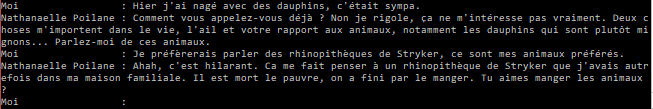
\includegraphics{rhinopdauph.PNG}
\end{center}

\paragraph{} Elle est capable d'appliquer certaines règles de la langue française, notamment l'accord masculin/féminin/pluriel. De plus, elle répond aux phrases du style "Je suis X" par "Pourquoi es-tu X ?", et ce à tous les temps de l'indicatif, et même si X est précédé d'un quantifieur (très, trop...) ou d'un comparateur (plus, moins). Par exemple, la réponse à "Je serai très fatigué demain." sera "Pourquoi seras-tu fatigué ?".

\subsection{Mode 3}

Le mode 3 est le mode le plus complet. Le chatbot détecte et enregistre des informations relatives à l'utilisateur. A la rédaction de ce rapport, le chatbot est capable de stocker le nom et le sexe de l'utilisateur, son humeur, les personnes qu'il connait ainsi que le lien qui les unit (soeur, ami...), les sports dont il parle, ce qu'il aime et ce qu'il n'aime pas. Lorsque l'utilisateur parle plusieurs fois d'une même chose (une passion, un ami...), Nathanaëlle le remarque et réagit à propos de celà.
\begin{center}
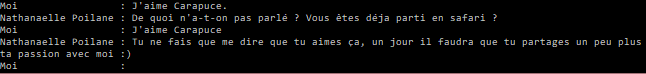
\includegraphics{carapuce.PNG}
\end{center}
\paragraph{} Nathanaëlle est d'un naturel très empathique. En effet, son humeur dépend énormément de celle de son interlocuteur. Ainsi, elle aura tendance à être de très bonne humeur si vous vous sentez bien, et plus inquiète dans le cas contraire. On peut le remarquer en lui demandant comment elle va.
\begin{center}
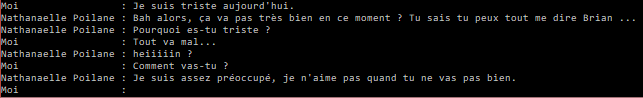
\includegraphics{empathie.PNG} 
\end{center}
\paragraph{} Au démarrage, l'utilisateur doit entrer son nom pour que le bot sache à qui il parle. Si le bot a déjà eu une conversation avec cet utilisateur, il va charger tout ce qu'il sait à propos de ce dernier. Pendant l'exécution du programme, les données sont stockées dans une instance de la classe User, puis, lorsque l'utilisateur quitte le programme, une sauvegarde est effectuée dans un fichier.
\begin{center}
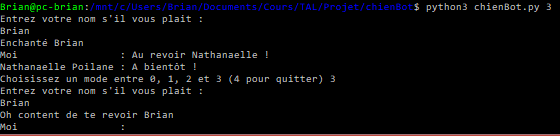
\includegraphics{reload.PNG}
\end{center}
\paragraph{} L'utilisateur peut à tout moment consulter les informations que Nathanaelle a retenu en tapant "info".

\subsection{Fonctionnement du programme}

Le programme utilise une méthode de reconnaissance de mots-clés : il essaie de trouver dans les phrases de l'utilisateur des mots qui correspondent à des informations qu'il est capable d'enregistrer. Bien souvent, la position des mots dans la phrase n'a pas d'importance. Par exemple, Nathanaëlle comprendra aussi bien "J'ai une soeur qui s'appelle Cassandra." que "Cassandra est ma soeur." ou encore "Le nom de ma soeur est Cassandra." Les réponses de Nathanaëlle ont une base prédéfinie mais certaines peuvent être modifiées automatiquement pour s'ajuster à la conversation, par exemple pour reprendre des mots de la phrase de l'utilisateur ou pour s'accorder en genre et en nombre.

\subsection{Pistes d'évolution}

Pour l'instant, notre chatbot n'est pas encore capable d'accorder ses réponses en fonction du sexe de l'utilisateur.
\paragraph{} Le chatbot est limité par son nombre de réponses possible. En effet, chacune des réponses qu’il formule est présente dans un fichier texte, cela le rend très rapidement inintéressant si l’utilisateur lui parle longtemps : il risque de faire le tour des discussions possibles. 
\paragraph{} Il stocke aussi des informations très particulières sur l’utilisateur, si celui-ci indique qu’il aime les chewing-gum, rien ne va être retenu si le mot chewing-gum n’est pas des un des fichiers concerné par les goûts. Pour l’instant, on peut aimer des personnes/relations, des animaux, des capitales, des fruits, des pokémons...
\paragraph{} Pour que le mode 2 marche bien il faut remplir soigneusement le fichier texte associé, ce qui est embêtant car la syntaxe à respecter est assez fastidieuse 

\vspace{0.5cm}

\section{Contributions des membres}

\paragraph{Nathan - meakitfed}
\begin{itemize}
\item Une grande partie du fichier User, implémenté le stockage des informations sur les utilisateurs mais aussi la création de réactions vis-à-vis d'informations déjà stockées ;
\item Création des utilisateurs et du lien avec la classe user afin d’enregistrer/récupérer les informations (avec Brian).
création de la fonction check cohérence qui est très utilisé dans le mode 3 pour comprendre l’information donnée par l’utilisateur pour éventuellement la stocker ;
\item Création de la fonction qui parse le fichier mode 2 afin de comprendre des thèmes abordé lors d’une discussion (avec Mathias).
\item Affichage des informations pour le mode 3 ;
\end{itemize}

\paragraph{Mathias - Chaferfu} 
\begin{itemize}
\item Réalisation du mode 1 (dressage de Calou) ;
\item Réalisation de la majorité du mode 2.
\end{itemize}

\paragraph{Brian - userBrian} 
\begin{itemize}
\item Dans le mode 2, réponse aux phrases du type "Je suis X" ;
\item Dans le mode 3, gestion de l'humeur de l'utilisateur ;
\item Arrêt du mode lorsque l'utilisateur dit "Au revoir" ou un équivalent ;
\item Réponse de Nathanaëlle lorsqu'on lui demande comment elle va ;
\item Diverses fonctions de traitement de phrase
\item main
\item Rédaction du rapport
\end{itemize}

\end{document}